\section{Technique Overview}
\label{sec:overview}
 
This section provides a brief overview of the transformation verification
technique with each component algorithm further elaborated in the sections that follow.

\subsection{Symbolic Execution}

Our algorithm operates on the principle of symbolic execution. In order to
explain the concept of symbolic execution of a transformation, let us make an
analogy with program symbolic execution as introduced by King in his seminal
work ``\emph{Symbolic Execution and Program
Testing}''~\cite{DBLP:journals/cacm/King76}. According to King, a symbolic
execution of a program is a set of \emph{constraints} on that program's
\emph{input variables} called \emph{path conditions}. Each \emph{path condition}
describes a traversal of the conditional branching commands of that program. A
\emph{path condition} is symbolic in the sense it \emph{abstracts} as many
concrete executions as there are instantiations of the path condition's
variables that render the path condition's constrains true.

We can transpose this notion of symbolic execution to model transformations. The
analog of an input variable in the model transformation context are
\emph{metamodel classes, relations and attributes}. As program statements impose
constraints on input and output variables during symbolic execution,
transformation rules impose conditions on which metamodel elements are
instantiated during a concrete transformation execution, and how that
instantiation happens.
Such conditions, built from transformation rules, can then be used as the analog
of program \emph{path conditions} in the context of model transformations. In
fact, throughout this paper we also use the term
\emph{path condition} in the context of model transformation verification.

As in program symbolic execution, each transformation path condition
\emph{abstracts} as many concrete executions as there are input/output models
that satisfy them. We must not forget that in a model transformation, rules are
implicitly or explicitly scheduled. Such control and/or data dependencies must
also be taken into consideration during path condition construction. In what
follows we will examine in more detail how these symbolic execution principles can
apply to the verification of model transformations.

% The correspondence between the symbolic
% execution concepts for \emph{programs} and \emph{model transformations} is shown
% in table~\ref{tab:symb_exec_analogy}.
% 
% \begin{table}[h] \centering
% \begin{tabular}{|l|l|l|}
% \hline
% \rowcolor{Gray}
%  & Program & Transformation\\
% \rowcolor{Gray}
%  & Symbolic Execution & Symbolic Execution\\
% \hline
% \hline
% Abstraction Over & Sets of data values & Sets of models (graphs)\\
% \hline	
% Input Variables & Programming language variables & Metamodel classes,\\
%  & (int, string, float, etc) & relations and attributes\\
% \hline
% Constraints & Predicates on variables imposed by & Metamodel patterns imposed\\
% & assignment or conditional statements & by transformation rules\\
% \hline
% Path Conditions & Conjunction of predicates & Conjunction of metamodel\\
% & on variables & patterns\\
% \hline
% \end{tabular}
% \caption{\emph{Program} Symbolic Execution vs. \emph{Model Transformation} Symbolic Execution}
% \label{tab:symb_exec_analogy}
% \end{table}
% 
% \renewcommand{\baselinestretch}{1.5}
% 
% \bentley{Need to connect these section}

\subsection{DSLTrans Rule Sequences}

Transformations are composed of a set of rules, which are applied to the input
model in some sequence depending on the elements present in that model. 

However, the sequence of rules that define a transformation execution may be infinite, as rules in an arbitrary transformation language may be repeatedly applied. The transformation language used here,
DSLTrans, is constructed so that each sequence of rules is finite. DSLTrans is explored more fully in the next section. One
important property of DSLTrans to highlight here is that rules are executed layer-by-layer, so that
rules from layer 2 cannot execute before rules from layer 1. Figure~\ref{fig:dsltransformation2} shows an abstract transformation with four rules arranged on two layers.

\begin{figure}[h!]
	\centering
		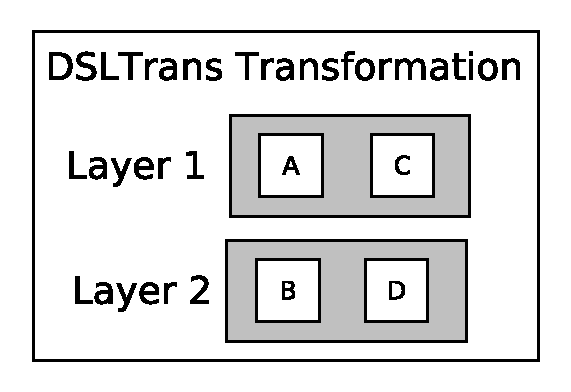
\includegraphics[width=0.4\textwidth]{./figures/overview/abstractDSLTransTransformation.pdf}
	\caption{An abstract DSLTrans model transformation}
	\label{fig:dsltransformation2}
\end{figure}

Each layer is composed of a set of transformation rules which execute in a
non-deterministic order but must produce a deterministic result. As the order of rule execution within a
layer will not matter, this drastically reduces the number of transformation rule sequences we need to examine. As well, DSLTrans transformations are not Turing-complete. As discussed in~\cite{DBLP:conf/sle/BarrocaLAFS10},
non-completeness is required to make rule sequences finite, but yet still allows
for appropriate expressiveness.

Besides the fact that DSLTrans' transformations are free of constructs that
imply unbounded recursion or non-determinism, DSLTrans' transformations are strictly outplace, meaning no changes are allowed
to the input model. However, the output metamodel for a DSLTrans transformation can
be the same as the input metamodel. Also, elements cannot be removed
from the output metamodel as the result of applying a DSLTrans rule.
This restriction is consistent with the usage of model transformations as
translations~\cite{AMT2012}, as no deletion of output elements is strictly required.

% This is
% however not the case when transformations are used to encode operational
% semantics (simulations) of systems~\levi{cite intent paper}. This illustrates the boundaries of the
% applicability of DSLTrans and that expressiveness reduction entails a compromise
% with the class of problems that can be tackled.

\subsection{Building Path Conditions}

As mentioned, a DSLTrans transformation will have rules structured in a number of layers, so as to define rule ordering. In order to create all possible path conditions defined by this transformation, path conditions will be created in a corresponding layer-by-layer manner. We provide a brief overview here, while a precise explanation follows in section~\ref{sec:building_pcs}.

\subsubsection{Rule Combinations}


In order to provide an intuition for path condition creation, we shall discuss a method to create path conditions for the first layer only. The technique is to produce all possible combinations of rules, using the powerset of rules. These rule combinations can then be made into path conditions by taking the union of all rules in that rule combination. Figure~\ref{fig:first_layer} shows how the possible rule combinations for a layer. 

\begin{figure}[h!]
	\centering
		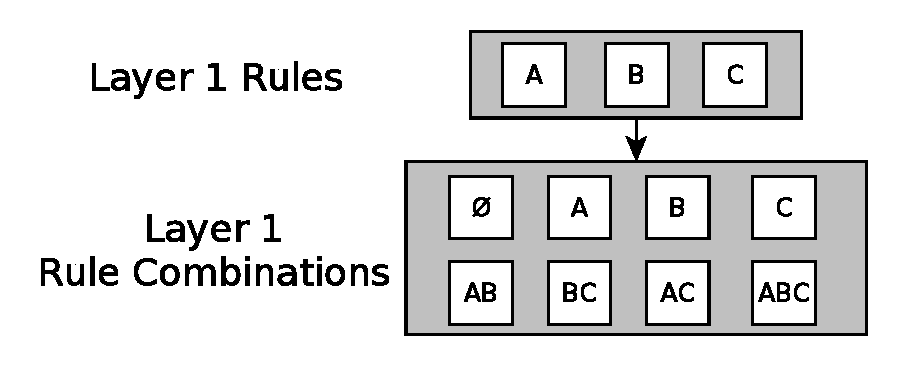
\includegraphics[width=0.5\textwidth]{./figures/overview/rule_combos.pdf}
	\caption{Creating path conditions through rule combinations}
	\label{fig:first_layer}
\end{figure}

An important characteristic of our technique is that the number of times a rule executes is abstracted over in a rule combination or path condition. If a rule's execution is represented by a path condition, the rule has executed one or more times. For instance, the example path condition \emph{AC} in Figure~\ref{fig:first_layer} represents all transformation executions where both rules A and C have executed one or more times, and rule B has not executed.


\subsubsection{Generating All Path Conditions}

The creation of path conditions through rule combinations is only a valid process for the first layer, and is mentioned solely as an explanatory tool. In further layers, DSLTrans rules may contain dependencies which prevent them from executing. Therefore, the algorithm must move layer-by-layer through the transformation, and determine which rules may execute.

The path condition generation algorithm begins by creating a set containing an empty path condition. This path condition represents all transformation executions where no rules have yet executed. The path condition is then sequentially combined with each rule from the first layer of the transformation. The combination process determines all the possible ways that the rule can be added to the path condition, as detailed in section~\ref{sec:building_pcs}.

For example, consider figure~\ref{fig:layers_pc}. The path condition PC at the top of the figure may either be the empty path condition, or a path condition from the previous layer. PC is then combined with a rule R1 
selected from the current layer. The path condition and rule may combine in different ways. For instance, the rule might not execute, in which case the path condition is left unchanged. Another case is that the rule does execute, in which case the rule is ``glued'' to the path condition in a particular way. This combination process will create one or more path conditions which take into account all possibilities of how the rule might execute.

In ~\ref{fig:layers_pc}, combining the path condition PC with rule 1 has produced three path conditions: the unchanged PC, and two different possibilities of how the rule combined with PC (denoted PC + R1 and PC + R1'). These three path conditions are then combined with rule 2. Three further path conditions are produced, representing transformation executions where rule 2 does not execute. As well, three path conditions are produced that represent transformation executions where rule 2 does execute.

%
%\begin{figure}[htb]
%\centering
%        \begin{subfigure}[b]{0.480\textwidth}
%                \centering
%                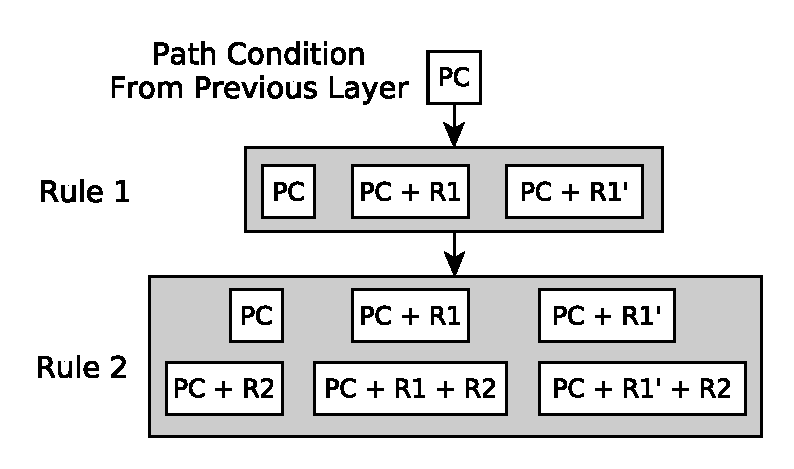
\includegraphics[width=1\textwidth]{./figures/overview/layers_pc.pdf}
%                 \caption{Combining a path condition with two rules}
%                 \label{fig:layers_pc}
%        \end{subfigure}%
%        ~~
%        \begin{subfigure}[b]{0.48\textwidth}
%                        \centering
%                        
%             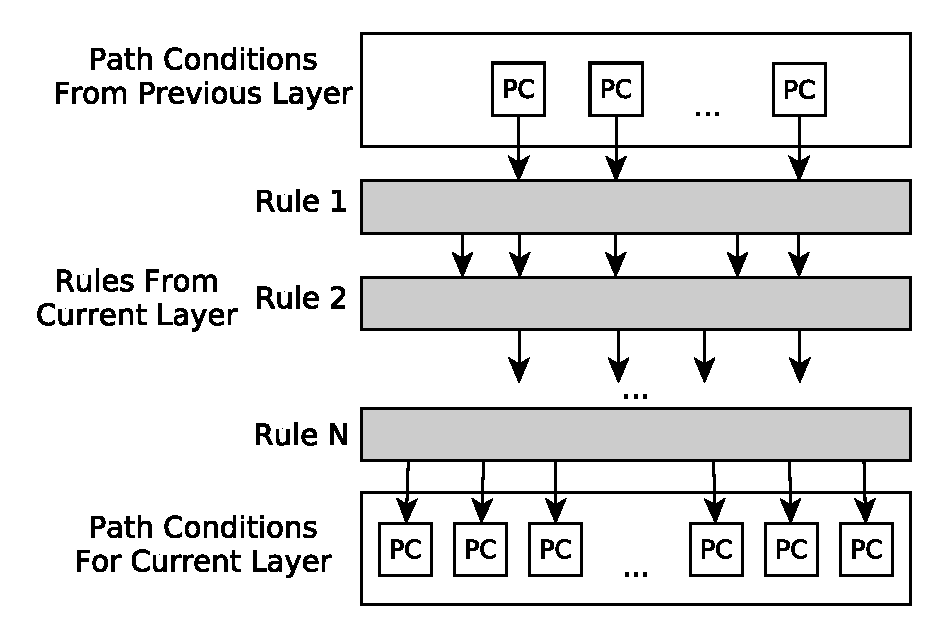
\includegraphics[width=1\textwidth]{./figures/overview/all_pcs.pdf}
%             \caption{Creating all path conditions for a layer}
%             \label{fig:all_pcs}
%	    \end{subfigure}%
%           \caption{Creating path conditions}
%         \label{fig:creating_pcs}
%\end{figure}


Rules in DSLTrans may also define dependencies in which elements have been previously created in the transformation. These dependencies further restrict the ways that a path condition and rule may combine. These dependencies are checked against the path condition from the previous layer, not the path combination the rule is to be combined with. This is to preserve the semantics of DSLTrans rules, where a rule cannot depend upon the output of another rule in the same layer.



Figure~\ref{fig:next_layer2} diagrams how the path condition generation process occurs layer-by-layer. The path conditions from the previous layer are combined with all the rules in the current layer, to produce a set of path conditions for the layer. This set will then be combined with the rules from the next layer of rules. After this process repeats for all layers in the transformation, the final set of path conditions is then used for property proving.

\begin{figure}[htb]
              
        \centering
        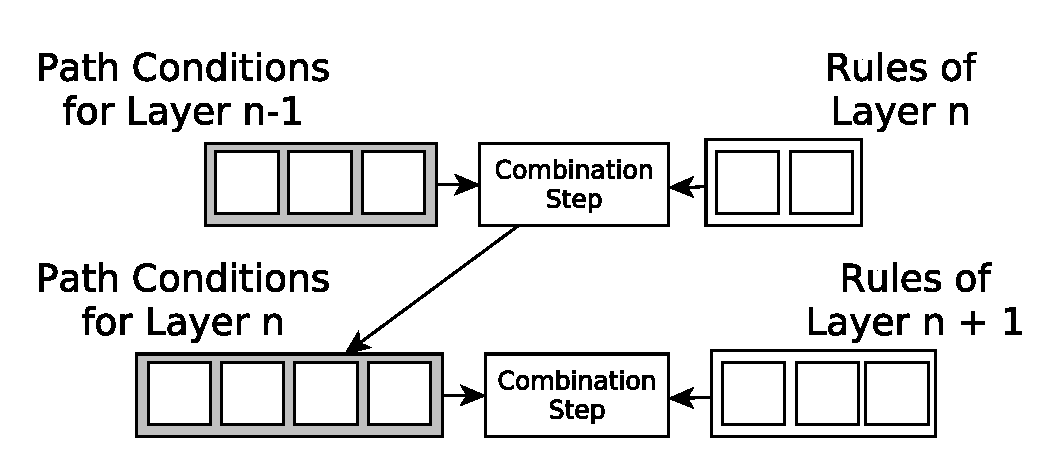
\includegraphics[width=0.8\textwidth]{./figures/building_path_conditions/next_layer.pdf}
        \caption{Path conditions are combined with rules in next layer}
        \label{fig:next_layer2}
\end{figure}

 
 
\subsection{Proving Properties}

The final set of path conditions produced will define all possible concrete transformation executions through an abstraction relation that we define in Definition~\ref{def:instance_pc_ex}. This abstraction relation allows us to prove properties on each path condition in the final path condition set and have that result hold on all transformation executions abstracted by that path condition. An overview of the property proving process is presented here, while further details as well as formal validity and completeness proofs are found in section~\ref{sec:verif_dsltrans_props}.

Path conditions are represented in much the same way as DSLTrans rules. This is because path conditions represent the interaction of a set of DSLTrans rules. Path conditions contain two graphs. The first graph represents a pattern that must be present in the input model of the transformation. The second is a pattern which will be instantiated in the output model of the transformation, including traceability to elements matched by the rules. The formal definition of a path condition can be seen in definition~\ref{def:path_condition}.

The properties we are interested in have an implication form. They represent the
following statement: if this pattern is found in the input model, then
this other pattern must be found in the output model, possibly including traceability constraints. Therefore,
we encode properties as a set of pre-condition and post-condition patterns.

Property proving then becomes relatively simple. The path condition match graph
represents the elements which define that path condition. Likewise, the property
pre-condition pattern represents the prerequisite for the property. Thus,
property proving algorithm will attempt to isomorphically find the property's
pre-condition pattern in the path condition's match graph. If not found, then the
property will not be validated on this path condition, as the prerequisites do
not exist.

If the property's pre-condition pattern is found, then the property's
post-condition pattern is isomorphically searched for in the path condition. If
it is found, then the rule execution defined by that path condition will produce
the required elements for that property and the property will hold. If not
found, then the necessary elements will not be produced and the property check
will fail.

In this way, all path conditions are checked to see if the property specified is
applicable to that execution, and then if the execution satisfies that property.
Therefore, properties can be verified for all possible executions of a
transformation using the abstraction relation.

Future chapters will examine each step of this algorithm in detail. Following this, results will be provided to indicate that our algorithm is feasible and can scale to industry-sized transformations.